\section{Влияние скорости охлаждения образца на результирующий профиль}

Важной особенность метода СЭЛТР является тот факт, что формирование профиля завершается только при охлаждении образца до температуры около 80~$^\circ$C, что занимает некоторое время после окончания экспонирования.
В данном разделе приводятся результаты моделирования конечного профиля линии, получаемой методом СЭЛТР, при значениях скорости охлаждения образца, отличающихся от скорости его охлаждения в эксперименте.

Как и ранее, считалось, что экспонирование резиста в процессе СЭЛТР производится ``в кадр'' с параметрами кадра, описанными в разделе~\ref{sec:verification}.
В качестве исходных параметров экспонирования были приняты $T$ = 130~$^\circ$C, $t_\mathrm{exp}$~=~100~c, $I$ = 4.56 нА, диаметр пучка составлял 600 нм, начальная толщина слоя ПММА -- 500 нм, зависимость температуры образца от времени при охлаждении изначально описывалась экспериментальной кривой охлаждения, приведенной на рисунке~\ref{fig:exp_cooling} (профиль линии, получаемой в этих условиях, приведен на рисунке~\ref{fig:DEBER_4_profiles}в).
При данных параметрах процесса СЭЛТР в слое ПММА на момент остывания присутствуют микрополости, что обеспечивает меньший радиус кривизны профиля в центре линии по отношению к случаю полного заполнения микрополостей (рисунки~\ref{fig:DEBER_4_profiles}а, \ref{fig:DEBER_4_profiles}б и \ref{fig:DEBER_4_profiles}г).

На рисунке~\ref{fig:DEBER_cooling} приведены промоделированные профили линий, полученных методом СЭЛТР при одинаковых условиях экспонирования, описанных выше, но с разными значениями скорости охлаждения образца после экспонирования.
Результаты моделирования демонстрируют заметное влияние микрополостей в слое резиста на форму профиля, особенно в центре линии.
Исходя из того, что среднеквадратичное отклонение точек промоделированных профилей в центре линии при наличии микрополостей составляет около 15 нм, требование к стабильности скорости охлаждения образца может быть сведено к максимально допустимой флуктуации скорости охлаждения образца, равной 0.1~$^\circ$C/с (данное значение получено аналогично максимально допустимым значениям флуктуаций параметров экспонирования, приведенным ранее).

\begin{figure}[h]
	\begin{minipage}{0.48\textwidth}
		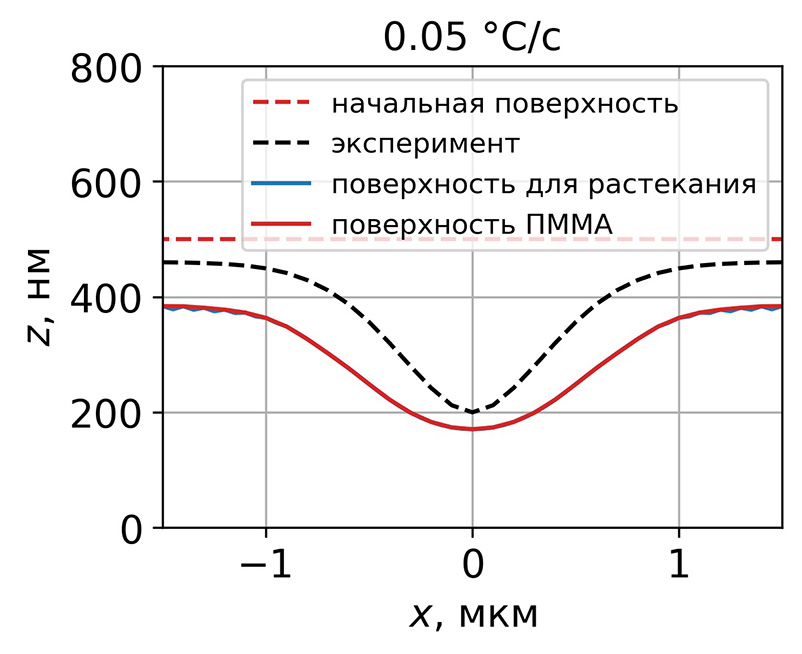
\includegraphics[width=\linewidth]{DEBER_cooling/cooling_0p05_200} \\
		\vspace{-13em} \\ \text{\hspace{0em} a}) \\ \vspace{13em}
	\end{minipage}
	\begin{minipage}{0.48\textwidth}
		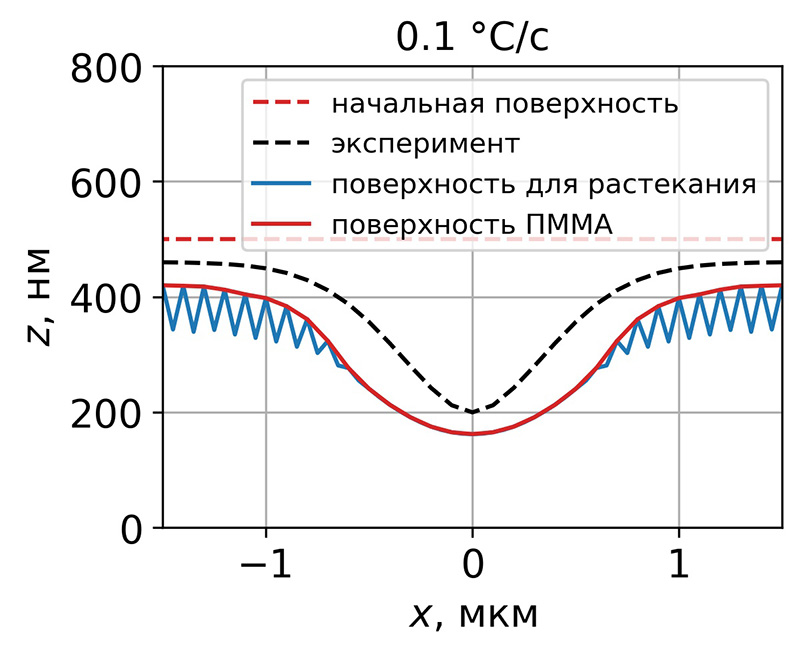
\includegraphics[width=\linewidth]{DEBER_cooling/cooling_0p1_200} \\
		\vspace{-13em} \\ \text{\hspace{-0.1em} б}) \\ \vspace{13em}
	\end{minipage}
	
	\vspace{-3em}
	
	\begin{minipage}{0.48\textwidth}
		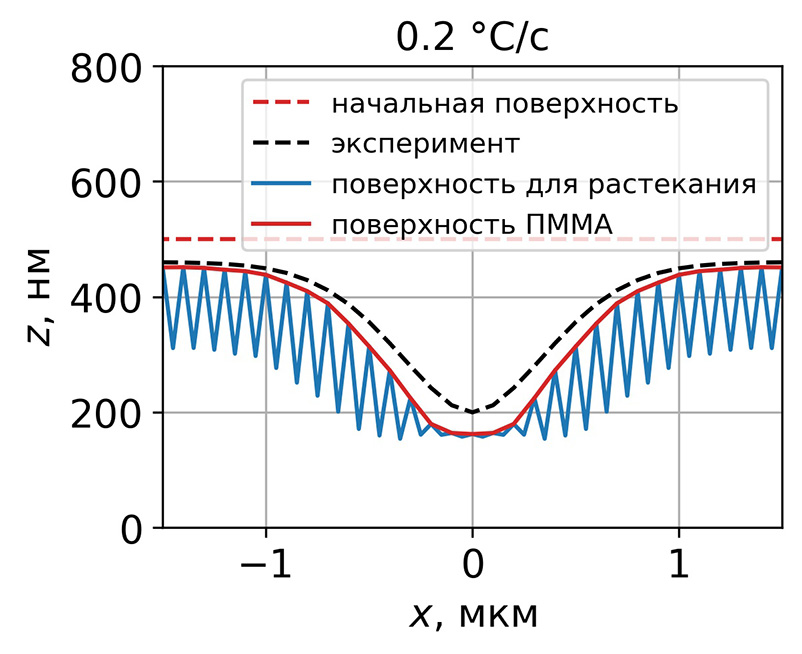
\includegraphics[width=\linewidth]{DEBER_cooling/cooling_0p2_200} \\
		\vspace{-13em} \\ \text{\hspace{0em} в}) \\ \vspace{13em}
	\end{minipage}
	\begin{minipage}{0.48\textwidth}
		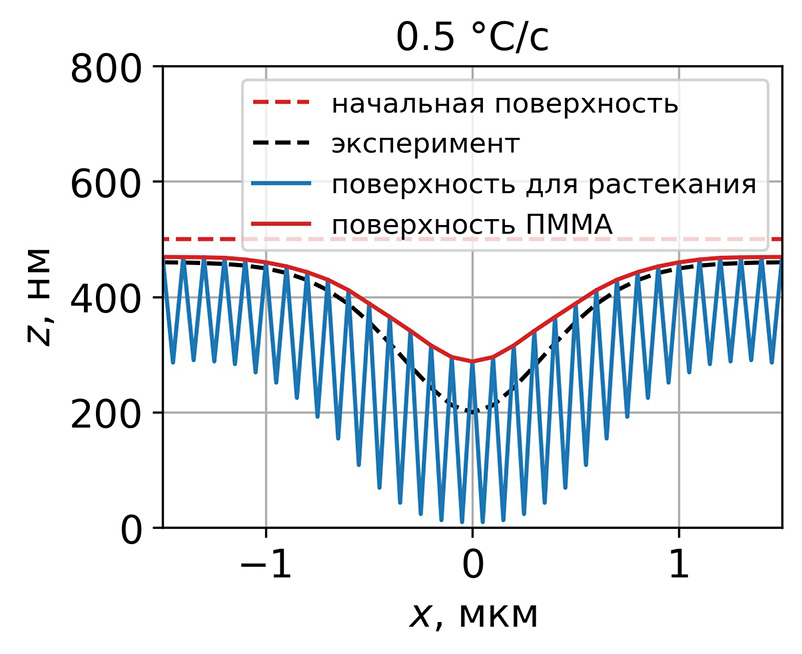
\includegraphics[width=\linewidth]{DEBER_cooling/cooling_0p5_200} \\
		\vspace{-13em} \\ \text{\hspace{-0.1em} г}) \\ \vspace{13em}
	\end{minipage}
	\vspace{-3em}
	\caption{Промоделированные профили, полученные методом СЭЛТР при $T$ = 130~$^\circ$C, $t_\mathrm{exp}$ = 100 c и $I$ = 4.56 нА. Скорость охлаждения образцов варьируется в пределах 0.05--0.5 $^\circ$C.}
	\label{fig:DEBER_cooling}
	\vspace{1em}
\end{figure}
